\documentclass[a4paper,12pt]{article}

% Packages
\usepackage[utf8]{inputenc} % For UTF-8 encoding
\usepackage[hungarian]{babel} % Hungarian language support
\usepackage{amsmath, amssymb} % Math symbols and environments
\usepackage{geometry} % Page geometry
\usepackage{titlesec} % Section formatting
\usepackage{enumitem} % Custom lists
\usepackage{hyperref} % Hyperlinks
\usepackage{fancyhdr} % Header and footer customization
\usepackage{graphicx} % Include graphics
\usepackage{multirow}
\usepackage{tikz}
\usepackage{pgfplots}
\usepgfplotslibrary{statistics}



% Page settings
\geometry{margin=1in}

% Title and author
\title{\textbf{Biostatisztika Záróvizsga Tételek}}
\author{Név: \textit{[Pinczés Dániel]}}
\date{\today}

% Header and footer
\pagestyle{fancy}
\fancyhf{}
\lhead{Záróvizsga Tételek}
\rhead{\thepage}

% Section formatting
\titleformat{\section}[block]{\bfseries\Large}{Tétel \thesection}{1em}{}
\titleformat{\subsection}[block]{\bfseries\large}{\thesubsection}{1em}{}

\begin{document}

% Title Page
    \maketitle
    \thispagestyle{empty}
    \newpage

% Table of Contents
    \tableofcontents
    \newpage

% Example Sections for Topics


    \section{A biostatisztika áttekintése: kérdésfeltevések és alapproblémák}

    \textbf{Tétel}:

    Tipikus problémák a biostatisztikában, a matematikailag megalapozott módszerek
    szükségessége az orvosbiológiai kutatások támogatásában. A humán empirikus orvosi
    kutatások módszerei, kísérlet és megfigyelés. A confounding fogalma. Védekezési
    lehetőségek a confounding ellen.

    \subsection{Tipikus problémák a biostatisztikában, a matematikailag megalapozott módszerek
    szükségessége az orvosbiológiai kutatások támogatásában.}
    Itt található az első tételhez tartozó első alcím részletezése.

    A biostatisztika az orvosi és biológiai kutatásokban felmerülő statisztikai kérdésekkel foglalkozik. Az "Az orvosi megismerés módszertana" című könyv számos példát hoz olyan kérdésekre, amelyek tipikusan előfordulnak az orvosi kutatásokban, és amelyek megválaszolásához statisztikai módszerekre van szükség. Ezek a kérdések általában ok-okozati összefüggések feltárására irányulnak.

    \begin{itemize}
        \item Környezeti tényezők és egészségügyi hatások

        "Okoz-e mentális betegséget a légszennyezettség?" (Forrás: 2. fejezet, 15. oldal) Ez a kérdés rávilágít arra, hogy a biostatisztikában gyakran vizsgálunk olyan problémákat, ahol egy környezeti tényező (jelen esetben a légszennyezettség) potenciális egészségügyi hatását szeretnénk felmérni.

        \item Technológiai fejlődés és egészségügyi kockázatok

        "A mobiltelefon-használat okoz-e agydaganatot?" (Forrás: 2. fejezet, 15. oldal) Ez a példa azt mutatja, hogy a biostatisztika fontos szerepet játszik az új technológiák potenciális egészségügyi kockázatainak értékelésében.

        \item Életmódbeli tényezők és betegségek kapcsolata

        "A vöröshús-fogyasztás növeli-e a vastagbélrák kockázatát?" (Forrás: 2. fejezet, 15. oldal) Ez a kérdés rámutat arra, hogy a biostatisztika gyakran foglalkozik olyan problémákkal, amelyek az életmód és a betegségek közötti összefüggéseket vizsgálják.

        \item Orvosi beavatkozások hosszú távú hatásai

        "A császármetszéssel születés növeli-e az 1-es típusú cukorbetegség kockázatát?" (Forrás: 2. fejezet, 15. oldal) Ez a példa azt illusztrálja, hogy a biostatisztika fontos szerepet játszik az orvosi beavatkozások hosszú távú következményeinek értékelésében.


        \item Gyógyszerek hatékonyságának vizsgálata

        "Egy új vérnyomáscsökkentő gyógyszer tényleg csökkenti-e a vérnyomást?" (Forrás: 2. fejezet, 15-16. oldal) Ez a kérdés rávilágít arra, hogy a biostatisztika kulcsfontosságú a gyógyszerek hatékonyságának és biztonságosságának értékelésében.

    \end{itemize}

    Az "Az orvosi megismerés módszertana" című könyv hangsúlyozza, hogy a matematikailag megalapozott módszerek elengedhetetlenek az orvosbiológiai kutatások támogatásában. Ennek több oka is van:

    \begin{itemize}

        \item Az empirikus megfigyelések önmagukban félrevezetőek lehetnek

        A könyv rámutat, hogy pusztán a megfigyelésekre hagyatkozva téves következtetésekre juthatunk. Erre kiváló példa az érvágás esete, amelyet a könyv részletesen tárgyal. Az érvágást évszázadokon át alkalmazták különböző betegségek gyógyítására, anélkül, hogy bárki empirikusan megvizsgálta volna annak tényleges hatásosságát. (Forrás: 1. fejezet, 8-10. oldal)

        \item A véletlen ingadozás hatásának kezelése:

        A könyv kifejti, hogy az orvosi kutatásokban mindig jelen van a véletlen ingadozás. Ez azt jelenti, hogy még akkor is kaphatunk eltérő eredményeket, ha valójában nincs valódi különbség vagy hatás. A matematikai módszerek segítenek abban, hogy megkülönböztessük a valódi hatásokat a véletlen ingadozásoktól. (Forrás: 5. fejezet, 47-48. oldal)

        \item Ok-okozati összefüggések feltárása

        A könyv hangsúlyozza, hogy az ok-okozati összefüggések feltárása komplex feladat. Nem elég csupán azt megállapítani, hogy két jelenség együtt jár, azt is ki kell mutatni, hogy az egyik okozza a másikat. Ehhez szükség van olyan matematikai módszerekre, amelyek képesek kezelni a zavaró tényezőket (confoundereket) és más komplex összefüggéseket. (Forrás: 2. fejezet, 16-17. oldal)

        \item A mintavételi hiba kezelése

        A könyv rámutat, hogy a kutatások során általában csak egy mintát tudunk vizsgálni, nem a teljes populációt. A matematikai módszerek segítenek abban, hogy a mintából nyert eredményeket megfelelően tudjuk általánosítani a teljes populációra. (Forrás: 5. fejezet, 64-65. oldal)

        \item A kutatások tervezése

        A matematikailag megalapozott módszerek nem csak az adatok elemzésében, hanem már a kutatások tervezésében is kulcsfontosságúak. A könyv részletesen tárgyalja, hogyan lehet meghatározni a szükséges mintaméretet, vagy hogyan lehet randomizálni a résztvevőket egy klinikai vizsgálatban. (Forrás: 5. fejezet, 68-71. oldal)

        \item A bizonytalanság számszerűsítése

        A könyv kiemeli, hogy a matematikai módszerek lehetővé teszik a bizonytalanság számszerűsítését. Ez segít abban, hogy ne csak azt tudjuk meg, mi a legjobb becslésünk egy hatás nagyságára, hanem azt is, mennyire lehetünk biztosak ebben a becslésben. (Forrás: 5. fejezet, 53-55. oldal)

    \end{itemize}

    A könyv konkrét példaként említi James Lind skorbut elleni kísérletét és Pierre-Charles-Alexandre Louis érvágással kapcsolatos vizsgálatát, amelyek a szisztematikus, empirikus vizsgálatok fontosságát demonstrálják. (Forrás: 1. fejezet, 10-11. oldal)

    Saját kiegészítés: Fontos megjegyezni, hogy a matematikailag megalapozott módszerek nem helyettesítik, hanem kiegészítik az orvosi szakértelmet. A statisztikai eredmények értelmezéséhez és a klinikai gyakorlatba való átültetéséhez továbbra is szükség van az orvosok szakértelmére és tapasztalatára. A matematikai módszerek inkább eszközök, amelyek segítik az orvosokat a jobb döntéshozatalban és a tudományos bizonyítékok értékelésében.

    \subsection{A humán empirikus orvosi kutatások módszerei, kísérlet és megfigyelés}

    Az orvosi kutatásokban két fő módszert különböztetünk meg az empirikus vizsgálatok során: a kísérletet és a megfigyelést. A könyv részletesen tárgyalja mindkét módszert, kiemelve azok előnyeit és hátrányait.

    \subsubsection{Kísérlet}

    A kísérlet során a kutatók aktívan befolyásolják az expozíciót, vagyis azt a tényezőt, amelynek a hatását vizsgálni szeretnék.

    \begin{itemize}

        \item \textbf{Jellemzői}: A kutatók döntik el, ki kerül a kezelt és ki a kontroll csoportba. Lehetővé teszi a randomizációt, ami a leghatékonyabb módszer a confounding ellen. Általában kisebb mintamérettel dolgozik, mint a megfigyeléses vizsgálatok. Az utánkövetési idő gyakran korlátozott.

        \item \textbf{Példa}: James Lind skorbut elleni kísérlete, ahol a tengerészeket különböző csoportokba osztotta, és eltérő kezeléseket alkalmazott. (Forrás: 1. fejezet, 11. oldal)

        \item \textbf{Előnyök}: Lehetővé teszi az ok-okozati összefüggések közvetlen vizsgálatát.
        A randomizáció révén kiküszöböli a confounding hatását.

        \item \textbf{Hátrányok}: Etikai korlátok (pl. nem lehet szándékosan káros expozíciónak kitenni az alanyokat).
        Költséges és időigényes lehet.
        A résztvevők összetétele gyakran eltér a teljes populációétól. (Forrás: 3. fejezet, 27-30. oldal)

    \end{itemize}

    \subsubsection{Megfigyelés}

    A megfigyeléses vizsgálatok során a kutatók nem befolyásolják az expozíciót, csak megfigyelik és rögzítik az eseményeket.

    \begin{itemize}

        \item \textbf{Jellemzői}: A kutatók nem avatkoznak be az expozíció kiosztásába.
        Általában nagyobb mintamérettel dolgozik.
        Hosszabb utánkövetési idő lehetséges.
        A vizsgált populáció jobban reprezentálja a teljes populációt.
        Példa: A légszennyezettség és a mentális betegségek kapcsolatának vizsgálata, ahol a kutatók nem befolyásolják, ki él szennyezett területen. (Forrás: 2. fejezet, 15. oldal)

        \item  \textbf{Előnyök}: Etikailag kevésbé problémás.
        Nagyobb mintaméret és hosszabb utánkövetési idő lehetséges.
        Jobban reprezentálja a valós életbeli körülményeket.

        \item \textbf{Hátrányok}: Nehezebb az ok-okozati összefüggések megállapítása.
        A confounding problémája jelentősebb.
    \end{itemize}


    (Forrás: 3. fejezet, 28-30. oldal)

    A könyv hangsúlyozza, hogy mindkét módszernek megvan a maga helye az orvosi kutatásokban. A kísérletek erőssége, hogy jobban kontrollálhatók és alkalmasabbak ok-okozati összefüggések feltárására. A megfigyeléses vizsgálatok viszont jobban tükrözik a valós életbeli körülményeket, és olyan helyzetekben is alkalmazhatók, ahol a kísérletek etikailag vagy gyakorlatilag nem kivitelezhetők.

    A könyv egy érdekes példát hoz az ejtőernyők hatékonyságának vizsgálatára, ami jól szemlélteti a kétféle módszer közötti különbséget és azok korlátait. (Forrás: 3. fejezet, 30-31. oldal)

    Saját kiegészítés: Fontos megjegyezni, hogy a modern orvosi kutatásokban gyakran kombinálják a kétféle megközelítést. Például egy megfigyeléses vizsgálat eredményei alapján hipotéziseket állítanak fel, amelyeket aztán klinikai kísérletekben tesztelnek. Vagy fordítva, egy klinikai kísérlet eredményeit későbbi megfigyeléses vizsgálatokkal validálják a való életben. Ez a kombinált megközelítés segít kihasználni mindkét módszer előnyeit, miközben minimalizálja azok hátrányait.

    \subsection{A confounding fogalma}

    A confounding (zavaró tényező) az orvosi kutatások egyik legfontosabb és leggyakoribb problémája. A könyv részletesen tárgyalja ezt a jelenséget, annak jelentőségét és következményeit.

    \textbf{Definíció}: A confounding olyan változó, amely egyszerre összefügg az expozícióval (a vizsgált tényezővel) és a végponttal (a vizsgált kimenetellel), ezáltal torzíthatja az eredményeket és hamis összefüggéseket sugallhat. (Forrás: 2. fejezet, 17-18. oldal)

    Példa a könyvből: A könyv egy szemléletes példát hoz a légszennyezettség és a mentális betegségek kapcsolatának vizsgálatára. Ebben az esetben a szocioökonómiai helyzet lehet confounder, mert:

    \begin{itemize}

        \item Összefügg az expozícióval

        A rosszabb szocioökonómiai helyzetű emberek gyakrabban élnek szennyezettebb területeken.

        \item Összefügg a végponttal

        A rosszabb szocioökonómiai helyzetű emberek körében gyakoribbak a mentális betegségek.

    \end{itemize}

    Így, ha csak a légszennyezettség és a mentális betegségek előfordulása közötti kapcsolatot vizsgáljuk, tévesen azt gondolhatjuk, hogy a légszennyezettség okozza a mentális betegségeket, holott valójában a szocioökonómiai helyzet állhat mindkettő hátterében. (Forrás: 2. fejezet, 17-20. oldal)

    \textbf{A confounding hatása}

    \begin{itemize}

        \item Hamis összefüggéseket mutathat ki
        Olyan kapcsolatot sugallhat két változó között, amely valójában nem létezik.


        \item Elfedheti a valódi összefüggéseket
        Elképzelhető, hogy van valódi kapcsolat két változó között, de a confounder miatt ezt nem tudjuk kimutatni.


        \item Torzíthatja a hatás nagyságát
        Még ha van is valódi kapcsolat, a confounder miatt túl- vagy alulbecsülhetjük annak mértékét.
    \end{itemize}

    A confounding felismerésének nehézségei: A könyv hangsúlyozza, hogy a confounding felismerése nem mindig egyszerű. Néha nyilvánvaló lehet (mint a fenti példában), de gyakran rejtett és nehezen azonosítható. Ráadásul egy vizsgálatban több confounder is jelen lehet egyidejűleg, tovább bonyolítva a helyzetet. (Forrás: 2. fejezet, 19-20. oldal)

    A confounding jelentősége: A könyv kiemeli, hogy a confounding figyelmen kívül hagyása súlyos következményekkel járhat. Téves következtetésekre juthatunk az ok-okozati összefüggésekről, ami helytelen klinikai döntésekhez vagy közegészségügyi intézkedésekhez vezethet. (Forrás: 2. fejezet, 20-23. oldal)

    Történeti példa: A könyv egy érdekes történeti példát is hoz a confounding problémájára. A 18. században Daniel Bernoulli azt vizsgálta, hogy miért magasabb a halálozási ráta a városokban, mint vidéken. Első ránézésre úgy tűnt, hogy a városi élet káros az egészségre. Azonban Bernoulli rájött, hogy az életkor egy confounder ebben az esetben: a városokba több fiatal költözött munkát keresni, és mivel a fiatalok általában egészségesebbek, ez torzította az összehasonlítást. (Forrás: 2. fejezet, 21-22. oldal)

    Saját kiegészítés: Fontos megjegyezni, hogy a confounding problémája nem csak az orvosi kutatásokban, hanem minden olyan területen jelentkezhet, ahol ok-okozati összefüggéseket próbálunk feltárni. Például a társadalomtudományokban, a pszichológiában vagy akár a gazdasági elemzésekben is kulcsfontosságú a zavaró tényezők azonosítása és kezelése. Az orvosi kutatásokban azért különösen kritikus ez a kérdés, mert a téves következtetések közvetlenül befolyásolhatják az emberek egészségét és életét.

    \subsection{Védekezési lehetőségek a confounding ellen}

    A könyv több módszert is ismertet, amelyekkel védekezhetünk a confounding hatása ellen. Ezek a módszerek segítenek abban, hogy pontosabb és megbízhatóbb következtetéseket vonhassunk le az orvosi kutatásokban.

    \subsubsection{Randomizáció}

    Ez a módszer kísérletes vizsgálatokban alkalmazható.

    \begin{itemize}
        \item \textbf{Lényege}
        A résztvevőket véletlenszerűen osztjuk be a különböző csoportokba (pl. kezelt és kontroll csoport).

        \item \textbf{Előnye}
        Ez a leghatékonyabb módszer, mert minden confoundert kiszűr, még azokat is, amelyekre nem gondoltunk.

        \item \textbf{Történeti példa}:
        James Burns Amberson 1931-es kísérlete, ahol pénzfeldobással döntötte el, hogy ki kapjon sanocrysin-t a TBC kezelésére.

        \item \textbf{Működési elv}:
        A randomizáció biztosítja, hogy a csoportok csak a vizsgált tényezőben (expozícióban) térjenek el egymástól, minden más szempontból hasonlóak legyenek.
        (Forrás: 3. fejezet, 26-27. oldal)

    \end{itemize}

    \subsubsection{Rétegzés}

    Ez a módszer megfigyeléses vizsgálatokban alkalmazható.

    \begin{itemize}
        \item \textbf{Lényege}: A confounding változó szerint rétegekre bontjuk a mintát, és rétegenként külön-külön végezzük el az elemzést.
        \item \textbf{Példa}: Ha az életkor a confounder, akkor külön vizsgáljuk az összefüggést a fiatalok, középkorúak és idősek csoportjában.
        \item \textbf{Előnye}: Egyszerű módszer, nem igényel bonyolult statisztikai eljárásokat.
        \item \textbf{Hátránya}: Ha sok confounder van, vagy folytonos változók (pl. életkor) esetén nehezen alkalmazható.
    \end{itemize}
    (Forrás: 4. fejezet, 33-35. oldal)

    \subsubsection{Standardizálás}

    Ez is megfigyeléses vizsgálatokban használatos módszer.

    \begin{itemize}
        \item \textbf{Lényege}: A confounding változó eloszlását egységesítjük a csoportok között, így téve összehasonlíthatóvá az eredményeket.
        \item \textbf{Példa}: A könyv részletesen tárgyalja a halálozási ráták standardizálását életkor szerint különböző országok összehasonlításakor.
        \item \textbf{Előnye}: Lehetővé teszi az összehasonlítást olyan esetekben is, amikor a csoportok összetétele nagyon eltérő.
        \item \textbf{Alkalmazás}: Gyakran használják epidemiológiai vizsgálatokban, például országok egészségügyi mutatóinak összehasonlításakor.
    \end{itemize}
    (Forrás: 4. fejezet, 35-43. oldal)

    \subsubsection{Többváltozós regressziós modellezés}

    A könyv említi, de részletesen nem tárgyalja ezt a módszert.

    \begin{itemize}
        \item \textbf{Lényege}: Statisztikai modelleket használunk, amelyek egyszerre több változó hatását tudják figyelembe venni.
        \item \textbf{Előnye}: Lehetővé teszi több confounder egyidejű kezelését.
        \item \textbf{Alkalmazás}: Széles körben használt módszer a modern orvosi kutatásokban.
    \end{itemize}

    (Forrás: 4. fejezet, 33. oldal)

    \subsubsection{Megfelelő kutatási terv}

    A könyv hangsúlyozza, hogy a confounding elleni védekezés már a kutatás tervezési fázisában elkezdődik.

    \begin{itemize}
        \item \textbf{Lényege}: Alapos előzetes tervezéssel azonosítjuk a potenciális confoundereket és beépítjük kezelésüket a kutatási tervbe.
        \item \textbf{Példa}: Adatgyűjtés során rögzítjük a releváns háttérváltozókat, amelyek később confounderként viselkedhetnek.
    \end{itemize}

    A könyv kiemeli, hogy a confounding kezelése kulcsfontosságú az orvosi kutatásokban, mert enélkül téves következtetésekre juthatunk az ok-okozati összefüggésekről. Ugyanakkor azt is hangsúlyozza, hogy a megfigyeléses vizsgálatokban soha nem lehetünk teljesen biztosak abban, hogy minden confoundert sikerült azonosítanunk és kezelnünk.

    Saját kiegészítés: Fontos megjegyezni, hogy a modern orvosi kutatásokban gyakran kombinálják ezeket a módszereket. Például egy megfigyeléses vizsgálatban alkalmazhatnak rétegzést és standardizálást is, majd az eredményeket többváltozós regressziós modellekkel ellenőrizhetik. Emellett az utóbbi években egyre nagyobb szerepet kapnak a fejlett statisztikai módszerek, mint például a propensity score matching vagy az instrumentális változók módszere, amelyek további lehetőségeket kínálnak a confounding kezelésére.


    \newpage


    \section{Az orvosi kutatások vizsgálati módszerei}

    \textbf{Tétel}:

    A vizsgálati módszerek csoportosítása. Megfigyeléses vizsgálatok: egyedi adatok alapuló
    vizsgálatok (kohorsz, eset-kontroll), aggregált adatokon alapuló (ecological) vizsgálatok,
    kontroll nélküli vizsgálatok. Kísérletes vizsgálatok jellemzői. Metaanalízisek fogalma, szerepe,
    fontossága.

    \subsection{A vizsgálati módszerek csoportosítása}

    Az "Az orvosi megismerés módszertana" című könyv alapján az orvosi kutatásokban alkalmazott vizsgálati módszereket alapvetően három fő csoportba sorolhatjuk:

    \textbf{Megfigyeléses vizsgálatok}
    \begin{itemize}
        \item A kutatók nem avatkoznak be az expozíció kiosztásába, csak megfigyelik és rögzítik az eseményeket.
        \item Ide tartoznak az egyedi és aggregált adatokon alapuló vizsgálatok, valamint a kontroll nélküli vizsgálatok.
    \end{itemize}

    \textbf{Kísérletes vizsgálatok}
    \begin{itemize}
        \item A kutatók aktívan befolyásolják az expozíciót.
        \item Lehetővé teszik a randomizációt és a kontrollált körülmények közötti vizsgálatot.
    \end{itemize}

    \textbf{Metaanalízisek}
    \begin{itemize}
        \item Több, azonos kérdést vizsgáló kutatás eredményeinek statisztikai összegzése.
        \item Nem új adatgyűjtésen, hanem meglévő kutatások szintézisén alapul.
    \end{itemize}

    A könyv hangsúlyozza, hogy mindegyik módszernek megvan a maga helye és szerepe az orvosi kutatásokban. A módszerek közötti választást befolyásoló fő tényezők:

    \begin{itemize}
        \item A kutatási kérdés jellege
        \item Etikai megfontolások
        \item Gyakorlati megvalósíthatóság
        \item Rendelkezésre álló erőforrások
    \end{itemize}

    (Forrás: 3. fejezet, 27-30. oldal)

    \subsection{Megfigyeléses vizsgálatok}

    A megfigyeléses vizsgálatok olyan kutatási módszerek, ahol a kutatók nem avatkoznak be az expozíció kiosztásába, hanem passzívan figyelik meg és rögzítik az eseményeket. A könyv több típusú megfigyeléses vizsgálatot is tárgyal:

    \subsubsection{Egyedi adatokon alapuló vizsgálatok}

    \begin{enumerate}[label=(\alph*)]

        \item Kohorsz vizsgálatok

        \begin{itemize}
            \item textbf{Definíció}: Egy populációt hosszabb időn át követnek, és figyelik, hogy kik betegszenek meg.

            \item \textbf{Jellemzők}: Prospektív jellegű (előre tekintő)
            Az expozíciótól haladnak a végpont felé
            Alkalmas ritka expozíciók vizsgálatára

            \item  \textbf{Előnyök}: Időbeli sorrend tisztázható, több végpont is vizsgálható

            \item \textbf{Hátrányok}: Hosszú idő, drága, nem alkalmas ritka betegségek vizsgálatára

            \item \textbf{Példa}: A Framingham Heart Study, amely 1948-ban kezdődött, és több ezer embert követett évtizedeken át, hogy azonosítsa a szív- és érrendszeri betegségek kockázati tényezőit. (Forrás: 4. fejezet, 34. oldal)
        \end{itemize}

        \item Eset-kontroll vizsgálatok
        \begin{itemize}

            \item \textbf{Definíció}: Beteg (eset) és nem beteg (kontroll) csoportokat hasonlítanak össze a múltbeli expozíciók tekintetében.

            \item \textbf{Jellemzők}: Retrospektív jellegű (visszatekintő). A végponttól haladnak az expozíció felé. Alkalmas ritka betegségek vizsgálatára.


            \item \textbf{Előnyök}: Gyors, olcsó, jó ritka betegségekre

            \item \textbf{Hátrányok}: Nehéz megfelelő kontrollcsoportot találni, emlékezeti torzítás lehetősége

            \item \textbf{Példa}: Richard Doll és Austin Bradford Hill dohányzás és tüdőrák kapcsolatát vizsgáló kutatása az 1950-es években. Tüdőrákos betegeket (esetek) hasonlítottak össze nem tüdőrákos emberekkel (kontrollok), és vizsgálták a dohányzási szokásaikat. (Forrás: 4. fejezet, 35. oldal)

        \end{itemize}
        (Forrás: 4. fejezet, 33-35. oldal)

    \end{enumerate}

    \subsubsection{Aggregált adatokon alapuló (ecological) vizsgálatok}

    \begin{itemize}

        \item  \textbf{Definíció}: Nem egyénekre, hanem csoportokra vonatkozó adatokat elemeznek.

        \item \textbf{Jellemzők}:
        Populáció szintű adatokat használnak
        Gyorsan és olcsón kivitelezhetők

        \item \textbf{Előnyök}: Nagy populációkat lehet vizsgálni, olcsó.

        \item \textbf{Hátrányok}: Ökológiai tévkövetkeztetés veszélye (amit csoportszinten látunk, nem feltétlenül igaz egyéni szinten)

        \item \textbf{Példa}: A könyv említi az országok közötti összehasonlításokat, például a halálozási ráták összehasonlítását különböző országokban. (Forrás: 4. fejezet, 38-41. oldal)


    \end{itemize}

    \subsubsection{Kontroll nélküli vizsgálatok}

    \begin{itemize}

        \item \textbf{Definíció}: Egyetlen csoport megfigyelése kontrollcsoport nélkül.

        \item \textbf{Jellemzők}:
        Általában egy beavatkozás előtti és utáni állapotot hasonlítanak össze

        \item \textbf{Előnyök}: Egyszerű, gyors

        \item \textbf{Hátrányok}: Nem lehet kiszűrni az időbeli trendek hatását, confounding problémája jelentős

        \item \textbf{Példa}
        A könyv nem ad konkrét példát erre a típusra, de megemlíti, hogy ezek általában egy beavatkozás előtti és utáni állapotot hasonlítanak össze.\textbf{Elméleti illusztráció}: Egy új gyógyszer hatásosságának vizsgálata magas vérnyomásban szenvedő betegeknél. A kutatók kiválasztanak egy csoport magas vérnyomású beteget, megmérik a vérnyomásukat, majd elkezdik adni nekik az új gyógyszert. Egy meghatározott idő után (pl. 3 hónap) újra megmérik a vérnyomásukat, és összehasonlítják a kezdeti értékekkel.

    \end{itemize}

    A könyv hangsúlyozza, hogy a megfigyeléses vizsgálatok fő előnye, hogy valós életbeli körülményeket tükröznek, és olyan helyzetekben is alkalmazhatók, ahol kísérletek etikailag vagy gyakorlatilag nem kivitelezhetők. Ugyanakkor a fő hátrányuk, hogy nehezebb az ok-okozati összefüggések megállapítása, és a confounding problémája jelentősebb.

    (Forrás: 4. fejezet, 33-43. oldal)

    Saját kiegészítés: Fontos megjegyezni, hogy a modern epidemiológiában egyre kifinomultabb statisztikai módszereket alkalmaznak a megfigyeléses vizsgálatok elemzésére, hogy minimalizálják a confounding és egyéb torzítások hatását. Ilyen módszerek például a propensity score matching vagy az instrumentális változók módszere. Ezek segíthetnek abban, hogy a megfigyeléses vizsgálatok eredményei megbízhatóbbak legyenek, bár természetesen nem helyettesíthetik teljesen a randomizált kísérleteket.

    \subsection{Kísérletes vizsgálatok jellemzői}

    \subsubsection{Definíció}
    Kísérletes vizsgálatokban a kutatók aktívan befolyásolják az expozíciót, vagyis azt a tényezőt, amelynek a hatását vizsgálni szeretnék.

    (Forrás: 3. fejezet, 27. oldal)

    \subsubsection{Fő jellemzők}

    \paragraph{Beavatkozás az expozícióba:}
    \begin{itemize}
        \item A kutatók döntik el, ki kerül a kezelt és ki a kontroll csoportba.
        \item Ez lehetővé teszi az ok-okozati összefüggések közvetlen vizsgálatát.
    \end{itemize}

    \paragraph{Randomizáció:}
    \begin{itemize}
        \item A résztvevőket véletlenszerűen osztják be a csoportokba.
        \item Ez a leghatékonyabb módszer a confounding kiküszöbölésére.
        \item Példa: James Burns Amberson 1931-es TBC-kísérlete, ahol pénzfeldobással döntötte el, ki kap kezelést.
    \end{itemize}

    (Forrás: 3. fejezet, 26. oldal)

    \paragraph{Kontrollcsoport használata:}
    \begin{itemize}
        \item Lehetővé teszi a kezelés hatásának összehasonlítását a kezelés nélküli állapottal.
        \item Gyakran placebo-kontrollt alkalmaznak.
    \end{itemize}

    \paragraph{Vakosítás:}
    \begin{itemize}
        \item Egyszeresen vak: a résztvevők nem tudják, melyik csoportba kerültek.
        \item Kettősen vak: sem a résztvevők, sem a kutatók nem tudják, ki melyik csoportban van.
        \item Célja a torzítások csökkentése.
    \end{itemize}

    \subsubsection{Előnyök és hátrányok}

    \paragraph{Előnyök:}
    \begin{itemize}
        \item Lehetővé teszi az ok-okozati összefüggések közvetlen vizsgálatát.
        \item A randomizáció révén kiküszöböli a confounding hatását.
        \item Jól kontrollált körülmények között vizsgálhatók a hatások.
    \end{itemize}

    \paragraph{Hátrányok:}
    \begin{itemize}
        \item Etikai korlátok (pl. nem lehet szándékosan káros expozíciónak kitenni az alanyokat).
        \item Költséges és időigényes lehet.
        \item A résztvevők összetétele gyakran eltér a teljes populációétól (szelekciós torzítás).
        \item Általában kisebb mintamérettel dolgozik, mint a megfigyeléses vizsgálatok.
        \item Az utánkövetési idő gyakran korlátozott.
    \end{itemize}

    (Forrás: 3. fejezet, 27-31. oldal)

    \subsubsection{Alkalmazási területek}
    \begin{itemize}
        \item Gyógyszervizsgálatok
        \item Új terápiás eljárások tesztelése
        \item Prevenciós stratégiák hatékonyságának vizsgálata
    \end{itemize}

    \subsubsection{Etikai megfontolások}
    \begin{itemize}
        \item Minden kísérletes vizsgálathoz etikai bizottsági engedély szükséges.
        \item A résztvevők tájékozott beleegyezése elengedhetetlen.
        \item A potenciális kockázatokat és előnyöket gondosan mérlegelni kell.
    \end{itemize}

    \subsubsection{Példák}
    \begin{itemize}
        \item James Lind skorbut elleni kísérlete (1747)
        \item Az ISIS-2 vizsgálat, amely az aszpirin és sztreptokináznak nevezett vérrögoldó hatását vizsgálta infarktusban (1988)
    \end{itemize}

    (Forrás: 3. fejezet, 27-31. oldal, 6. fejezet, 88-89. oldal)

    \subsection{Metaanalízisek fogalma, szerepe, fontossága}

    \subsubsection{Fogalom}
    A metaanalízis több, azonos kérdést vizsgáló kutatás eredményeinek statisztikai összegzése. Ez egy szisztematikus módszer, amely lehetővé teszi, hogy különböző vizsgálatok eredményeit együttesen értékeljük és vonjunk le következtetéseket.

    (Forrás: 3. fejezet, 29. oldal)

    \subsubsection{Szerepe}

    \paragraph{Bizonyítékok szintézise:}
    A metaanalízis lehetővé teszi, hogy egy adott kutatási kérdésről átfogóbb képet kapjunk, mint amit egyetlen vizsgálat eredményei alapján kaphatnánk.

    \paragraph{Statisztikai erő növelése:}
    Az egyes vizsgálatok eredményeinek összevonásával növelhető a statisztikai erő, ami különösen fontos lehet ritka események vagy kis hatások kimutatásánál.

    \paragraph{Ellentmondások feloldása:}
    Ha különböző vizsgálatok ellentmondó eredményeket mutatnak, a metaanalízis segíthet tisztázni az összképet.

    \paragraph{Új hipotézisek generálása:}
    Az összesített adatok elemzése során új összefüggések, hipotézisek merülhetnek fel.

    \subsubsection{Fontossága}

    \paragraph{Magasabb szintű bizonyíték:}
    A metaanalízisek az evidencia-alapú orvoslás hierarchiájában magasabb szinten állnak, mint az egyedi vizsgálatok. Ez azt jelenti, hogy erősebb bizonyítékot szolgáltatnak egy adott kérdésben.

    \paragraph{Klinikai döntéshozatal támogatása:}
    Az összesített eredmények segíthetnek az orvosoknak a legjobb kezelési módok kiválasztásában.

    \paragraph{Kutatási irányok meghatározása:}
    A metaanalízisek rámutathatnak olyan területekre, ahol további kutatásokra van szükség.

    \paragraph{Erőforrások hatékony felhasználása:}
    Ahelyett, hogy újabb és újabb hasonló vizsgálatokat végeznének, a kutatók a meglévő eredményeket szintetizálhatják, ami idő- és költséghatékony.

    \subsubsection{Korlátok és kihívások}
    A könyv megemlíti, hogy bár a metaanalízisek rendkívül hasznosak, vannak korlátaik is:

    \paragraph{Publikációs torzítás:}
    A negatív eredményű vizsgálatokat ritkábban publikálják, ami torzíthatja a metaanalízis eredményeit.

    \paragraph{Heterogenitás:}
    Az összevont vizsgálatok között lehetnek módszertani vagy populációs különbségek, amelyek megnehezítik az összehasonlítást.

    \paragraph{Minőségi kérdések:}
    A metaanalízis eredménye csak olyan jó lehet, mint az alapjául szolgáló vizsgálatok minősége.

    (Forrás: 3. fejezet, 29-30. oldal)

    \newpage

\section{Deskriptív statisztika: kategoriális változó(k) vizsgálata}

\paragraph{Tétel:} Analitikus módszerek kategoriális változó vizsgálatára: gyakorisági sor, gyakoriság, relatív
gyakoriság, módusz. Grafikus módszer kategoriális változó vizsgálatára: oszlop- és
kördiagram. Két kategoriális változó egyidejű vizsgálata, kereszttábla.

\subsection{Analitikus módszerek kategoriális változó vizsgálatára}

\subsubsection{Gyakorisági sor}
A gyakorisági sor a kategoriális változó lehetséges kimeneteit (kategóriáit) tartalmazza, együtt azzal, hogy az adott kimenet hányszor fordult elő az adatbázisban.
(Forrás: 19. oldal)

\begin{description}
\item[Példa:] Tekintsük egy kórház betegfelvételi osztályán egy nap alatt felvett betegek nemét:
\begin{center}
\begin{tabular}{|c|c|}
\hline
Nem & Gyakoriság \\
\hline
Férfi & 45 \\
Nő & 55 \\
\hline
\end{tabular}
\end{center}
Ez a táblázat a nem változó gyakorisági sora.
\end{description}

\subsubsection{Gyakoriság}
A gyakoriság az adott kategória előfordulásainak száma az adatbázisban. A statisztikában általában $f$-fel jelölik. Ha az $i$-edik kategória gyakoriságáról van szó, akkor $f_i$-vel jelölik.
(Forrás: 19. oldal)

\begin{description}
\item[Példa:] A fenti példában $f_{\text{férfi}} = 45$ és $f_{\text{nő}} = 55$.
\end{description}

\subsubsection{Relatív gyakoriság}
A relatív gyakoriság az abszolút gyakoriság osztva a mintanagysággal ($n$-nel). Azt mutatja meg, hogy egy kategóriába a megfigyelési egységek mekkora hányada esik. A relatív gyakoriságok összege mindig 1.
(Forrás: 19-20. oldal)

\begin{description}
\item[Példa:] A fenti példában a relatív gyakoriságok:
\begin{align*}
\text{Férfi: } & \frac{45}{100} = 0,45 \text{ vagy } 45\% \\
\text{Nő: } & \frac{55}{100} = 0,55 \text{ vagy } 55\%
\end{align*}
\end{description}

\subsubsection{Módusz}
A módusz a leggyakoribb kimenet, azaz az a kategória, amelyhez tartozó gyakoriság a legnagyobb az adatbázisban. Jelölése: Mo.
(Forrás: 20. oldal)

\begin{description}
\item[Példa:] A fenti példában a módusz a "Nő" kategória, mivel ennek a legnagyobb a gyakorisága (55).
\end{description}

\subsubsection{Kiegészítések}

\paragraph{Kumulált gyakoriság és kumulált relatív gyakoriság}
Bár a könyv itt nem említi, de ordinális kategoriális változók esetén értelmezhető a kumulált gyakoriság ($f'$) és a kumulált relatív gyakoriság ($g'$) fogalma is. Ezek adott kategóriáig összegzik a gyakoriságokat, illetve relatív gyakoriságokat.

\begin{description}
\item[Példa:] Tekintsük egy fájdalomcsillapító hatékonyságának értékelését:
\begin{center}
\begin{tabular}{|c|c|c|c|}
\hline
Értékelés & Gyakoriság & Kumulált gyakoriság & Kumulált relatív gyakoriság \\
\hline
Nem hatásos & 10 & 10 & 0,1 \\
Kissé hatásos & 30 & 40 & 0,4 \\
Közepesen hatásos & 40 & 80 & 0,8 \\
Nagyon hatásos & 20 & 100 & 1,0 \\
\hline
\end{tabular}
\end{center}
\end{description}

\paragraph{Mintanagyság}
A mintanagyságot általában $n$-nel jelölik, és ez a gyakoriságok összege: $\sum_{i=1}^n f_i = n$.
(Forrás: 19. oldal)

\begin{description}
\item[Példa:] A betegfelvételi példában $n = 45 + 55 = 100$.
\end{description}

\paragraph{Megoszlás}
A teljes relatív gyakorisági sort a statisztikusok gyakran a változó megoszlásának hívják.
(Forrás: 20. oldal)

\begin{description}
\item[Példa:] A betegfelvételi példában a nem változó megoszlása: 45\% férfi, 55\% nő.
\end{description}

\paragraph{Információtömörítés}
A könyv kiemeli, hogy kategoriális változók esetében a gyakorisági sor nem jár információveszteséggel, ami speciális eset a statisztikában.
(Forrás: 20. oldal)

\paragraph{Ordinális vs. nominális változók}
A könyv megjegyzi, hogy az ordinalitás csak annyit módosít a fentieken, hogy a gyakorisági sorban a kategóriák felsorolási sorrendje kötött lesz.
(Forrás: 20. oldal)

\paragraph{Medián ordinális változóknál}
Bár a könyv itt nem részletezi, de megemlíti, hogy ordinális esetben elvileg definiálható lenne a medián fogalma is, de használata nem tipikus.
(Forrás: 20. oldal)

\begin{description}
\item[Példa:] A fájdalomcsillapító példában a medián a "Közepesen hatásos" kategória lenne, mert ez az a kategória, amely felett és alatt is a megfigyelések fele található.
\end{description}

\subsection{Grafikus módszer kategoriális változó vizsgálatára}

A kategoriális változók grafikus elemzése lényegében a gyakorisági sor vizualizálását jelenti. Ennek két, gyakorlatban legtipikusabb eszköze az oszlopdiagram és a kördiagram.
(Forrás: 21. oldal)

\subsubsection{Oszlopdiagram}

Az oszlopdiagram a kategóriák gyakoriságát vagy relatív gyakoriságát oszlopok magasságával szemlélteti.
(Forrás: 21. oldal)

\begin{description}
\item[Példa:] Tekintsük egy kórház sürgősségi osztályán egy nap alatt ellátott betegek triage kategóriáit:

\begin{center}
\begin{tabular}{|c|c|}
\hline
Triage kategória & Betegek száma \\
\hline
Azonnali ellátás & 5 \\
Nagyon sürgős & 15 \\
Sürgős & 30 \\
Kevésbé sürgős & 40 \\
Nem sürgős & 10 \\
\hline
\end{tabular}
\end{center}

\begin{center}
\setlength{\unitlength}{0.5cm}
\begin{picture}(20,10)
\put(0,0){\line(1,0){20}}
\put(0,0){\line(0,1){10}}
\put(2,0){\line(0,1){1}}
\put(6,0){\line(0,1){3}}
\put(10,0){\line(0,1){6}}
\put(14,0){\line(0,1){8}}
\put(18,0){\line(0,1){2}}
\put(1,-1){A}
\put(5,-1){NS}
\put(9,-1){S}
\put(13,-1){KS}
\put(17,-1){NS}
\put(-1,5){20}
\put(-1,10){40}
\end{picture}
\end{center}

\small{A: Azonnali, NS: Nagyon sürgős, S: Sürgős, KS: Kevésbé sürgős, NS: Nem sürgős}

\end{description}

Az oszlopdiagram előnye, hogy könnyen értelmezhető és összehasonlítható a kategóriák gyakorisága. Mind abszolút, mind relatív gyakoriságok ábrázolhatók vele.
(Forrás: 21. oldal)

\subsubsection{Kördiagram}

A kördiagram a kategóriák relatív gyakoriságát körcikkek területével szemlélteti.
(Forrás: 21. oldal)

\begin{description}
\item[Példa:] Az előző példa adatait kördiagramon ábrázolva:

\begin{center}
\setlength{\unitlength}{0.5cm}
\begin{picture}(10,10)
\put(5,5){\circle{10}}
\put(5,5){\line(1,0){5}}
\put(5,5){\line(3,4){3}}
\put(5,5){\line(-1,0){5}}
\put(5,5){\line(0,-1){5}}
\put(5,5){\line(4,-3){4}}
\put(7,8){5\%}
\put(9,5){15\%}
\put(7,2){30\%}
\put(2,2){40\%}
\put(2,7){10\%}
\end{picture}
\end{center}

\end{description}

A kördiagram előnye, hogy jól szemlélteti az egyes kategóriák arányát az egészhez képest. Hátránya, hogy csak relatív gyakoriságok ábrázolására alkalmas.
(Forrás: 21. oldal)

\subsubsection{Összehasonlítás és ajánlások}

A könyv megjegyzi, hogy tudományos munkákban általában az oszlopdiagram a preferált. Ennek oka, hogy pszichológiai vizsgálatok szerint az emberi szem jobban tud lineáris mértékeket kezelni és értelmezni, mint területet.
(Forrás: 21. oldal)

Az egyetlen megfontolás, ami mégis az oszlopdiagram ellen szólhat néha, hogy az oszlopok kirajzolási sorrendje már implikál egyfajta sorrendezést (a természetes balról-jobbra olvasás miatt), ami adott esetben nem következik az változó tartalmából.
(Forrás: 21. oldal)

\subsubsection{Ordinális változók esetén}

Az ordinalitás e téren nem sok változást okoz: az oszlopok sorrendje kötött lesz, illetve ábrázolhatóvá válik a kumulált gyakoriság is (természetesen csak oszlopdiagrammal).
(Forrás: 21. oldal)

\begin{description}
\item[Példa:] Az előző példában a triage kategóriák ordinális változót alkotnak. Ebben az esetben az oszlopdiagramon a kategóriák sorrendje kötött lenne (a sürgősség csökkenő sorrendjében), és ábrázolható lenne a kumulált gyakoriság is.
\end{description}

\subsection{Két kategoriális változó egyidejű vizsgálata, kereszttábla}

Két kategoriális változó kapcsolatának vizsgálatára a legfontosabb eszköz a kereszttábla (más néven kontingenciatábla vagy kombinációs tábla).
(Forrás: 33-34. oldal)

\subsubsection{Kereszttábla definíciója}

A kereszttábla egy olyan táblázat, melynek soraiban és oszlopaiban a két változó lehetséges kimenetelei vannak, az egyes cellákban pedig azon megfigyelési egységek darabszáma (tehát gyakorisága), melyek a cella sora és oszlopa szerinti kimenetűek a sorhoz illetve az oszlophoz rendelt változó szerint.
(Forrás: 33. oldal)

\begin{description}
\item[Példa:] Tekintsük egy kórházban felvett betegek nemét és dohányzási szokásait:

\begin{center}
\begin{tabular}{|c|c|c|c|}
\hline
\multicolumn{2}{|c|}{} & \multicolumn{2}{c|}{Dohányzás} \\
\cline{3-4}
\multicolumn{2}{|c|}{} & Igen & Nem \\
\hline
\multirow{2}{*}{Nem} & Férfi & 30 & 20 \\
\cline{2-4}
 & Nő & 15 & 35 \\
\hline
\end{tabular}
\end{center}

\end{description}

\subsubsection{Kereszttábla elemzése}

A kereszttáblából különböző típusú gyakoriságokat és relatív gyakoriságokat számolhatunk:

\paragraph{Abszolút gyakoriságok:} Ezek a táblázat celláiban szereplő számok.

\paragraph{Relatív gyakoriságok:} Az abszolút gyakoriságokat elosztjuk a teljes mintanagysággal.

\paragraph{Feltételes relatív gyakoriságok:} Az abszolút gyakoriságokat elosztjuk a megfelelő sor- vagy oszlopösszeggel.

\begin{description}
\item[Példa:] A fenti táblázatban:
\begin{itemize}
    \item Abszolút gyakoriság: pl. 30 (dohányzó férfiak száma)
    \item Relatív gyakoriság: pl. 30/100 = 0,3 (dohányzó férfiak aránya a teljes mintában)
    \item Feltételes relatív gyakoriság: pl. 30/50 = 0,6 (dohányzók aránya a férfiak között)
\end{itemize}
\end{description}

\subsubsection{Kapcsolat vizsgálata}

A kereszttábla segítségével vizsgálhatjuk a két változó közötti kapcsolatot. Két változó között akkor van kapcsolat, ha a sorváltozó feltételes megoszlásai különböznek az oszlopváltozó különböző értékei esetén (vagy fordítva).
(Forrás: 35-36. oldal)

\begin{description}
\item[Példa:] A fenti táblázatban kapcsolat látszik a nem és a dohányzási szokások között, mert:
\begin{itemize}
    \item A férfiak között a dohányzók aránya: 30/50 = 60\%
    \item A nők között a dohányzók aránya: 15/50 = 30\%
\end{itemize}
Ez arra utal, hogy a nemnek és a dohányzási szokásoknak van kapcsolata ebben a mintában.
\end{description}

\subsubsection{Mutatószámok}

A kapcsolat erősségének mérésére különböző mutatószámokat használhatunk, például:

\begin{itemize}
    \item Phi-együttható (2x2-es táblák esetén)
    \item Cramer's V (általános esetben)
    \item Kontingencia-együttható
\end{itemize}

Ezek a mutatók 0 és 1 között mozognak, ahol 0 jelenti a kapcsolat hiányát, 1 pedig a tökéletes kapcsolatot.
(Forrás: 37. oldal)

\subsubsection{Grafikus ábrázolás}

Két kategoriális változó kapcsolatát vizuálisan is megjeleníthetjük, például mozaikábrával vagy asszociációs ábrával, bár ezek nem olyan gyakoriak, mint az egyváltozós elemzéseknél használt oszlop- vagy kördiagramok.
(Forrás: 37-38. oldal)

\newpage

\section{Deskriptív statisztika: folytonos változó(k) vizsgálata}

\paragraph{Tétel:} Analitikus módszerek folytonos változó vizsgálatára: átlag, medián, terjedelem, szórás, IQR,
kvantilisek. Grafikus módszer folytonos változó vizsgálatára: hisztogram, magfüggvényes
sűrűségbecslés, Tukey-féle boxplot. Két folytonos változó együttes vizsgálata: kovariancia,
korreláció, szóródási diagram.

\subsection{Analitikus módszerek folytonos változó vizsgálatára}

A folytonos változók vizsgálatára számos analitikus módszer áll rendelkezésünkre. Ezek közül a legfontosabbak az alábbiak:

\subsubsection{Átlag}

Az átlag a centrális tendencia legismertebb mutatója. Definíció szerint:

\begin{equation}
\bar{x} = \frac{\sum_{i=1}^n x_i}{n}
\end{equation}

ahol $x_i$ az egyes megfigyelések, $n$ pedig a mintaelemszám.
(Forrás: 24. oldal)

\begin{description}
\item[Előnyök:] Közismert, könnyen értelmezhető.
\item[Hátrányok:] Nem robusztus, érzékeny a kiugró értékekre.
\end{description}

\subsubsection{Nyesett (trimmelt) átlag}

A nyesett átlag egy robusztusabb alternatívája a hagyományos átlagnak. Kiszámításához elhagyjuk a legkisebb és legnagyobb adott számú elemet, és csak a maradékot átlagoljuk.

\begin{equation}
\bar{x}_{\text{trim}} = \frac{\sum_{i=k+1}^{n-k} x_{(i)}}{n-2k}
\end{equation}

ahol $x_{(i)}$ a rendezett minta $i$-edik eleme, és $k$ az elhagyott elemek száma mindkét végén.

\begin{description}
\item[Előnyök:]
\begin{itemize}
    \item Robusztusabb, mint a hagyományos átlag
    \item Kevésbé érzékeny a kiugró értékekre
\end{itemize}
\item[Hátrányok:]
\begin{itemize}
    \item Nem használja fel az összes adatot
    \item A nyesés mértékének megválasztása szubjektív lehet
\end{itemize}
\end{description}

Tipikusan az 5\%-os trimmelt átlagot használják, ami azt jelenti, hogy a minta legkisebb és legnagyobb 5-5\%-át hagyják el.

(Forrás: 25. oldal)

\subsubsection{Medián}

A medián a nagyság szerint sorbarendezett megfigyelések közül a középső.

\begin{description}
\item[Előnyök:] Robusztus, nem érzékeny a kiugró értékekre.
\item[Hátrányok:] Kevésbé ismert, mint az átlag.
\end{description}

(Forrás: 25. oldal)

\subsubsection{Terjedelem}

A terjedelem a legnagyobb és a legkisebb mintaelem különbsége:

\begin{equation}
R = \max(x_i) - \min(x_i)
\end{equation}

\begin{description}
\item[Előnyök:] Egyszerű, könnyen értelmezhető.
\item[Hátrányok:] Nagyon érzékeny a kiugró értékekre.
\end{description}

(Forrás: 27. oldal)

\subsubsection{Szórás}

A szórás a megfigyelések átlagtól való átlagos eltérését méri:

\begin{equation}
s_x = \sqrt{\frac{\sum_{i=1}^n (x_i - \bar{x})^2}{n-1}}
\end{equation}

\begin{description}
\item[Előnyök:] Széles körben használt, jól interpretálható.
\item[Hátrányok:] Nem robusztus, érzékeny a kiugró értékekre.
\end{description}

(Forrás: 27. oldal)

\subsubsection{Interkvartilis terjedelem (IQR)}

Az IQR a harmadik és az első kvartilis különbsége:

\begin{equation}
IQR = Q_3 - Q_1
\end{equation}

\begin{description}
\item[Előnyök:] Robusztus, nem érzékeny a kiugró értékekre.
\item[Hátrányok:] Kevésbé ismert, mint a szórás.
\end{description}

(Forrás: 27-28. oldal)

\subsubsection{Kvantilisek}

A $p$-kvantilis az az érték, aminél a megfigyelések $p$-ed része kisebb, $(1-p)$-ed része nagyobb.

\begin{description}
\item[Speciális kvantilisek:]
\begin{itemize}
    \item Kvartilisek: $Q_1$ (25\%), $Q_2$ (50%, medián), $Q_3$ (75%)
    \item Decilisek: $D_1, D_2, ..., D_9$
    \item Percentilisek: $P_1, P_2, ..., P_{99}$
\end{itemize}
\end{description}

(Forrás: 26. oldal)

\subsection{Grafikus módszerek folytonos változó vizsgálatára}

\subsubsection{Hisztogram}

\begin{description}
\item[Példa:] Tekintsük 100 felnőtt személy vérnyomásának szisztolés értékét (Hgmm-ben).

\begin{center}
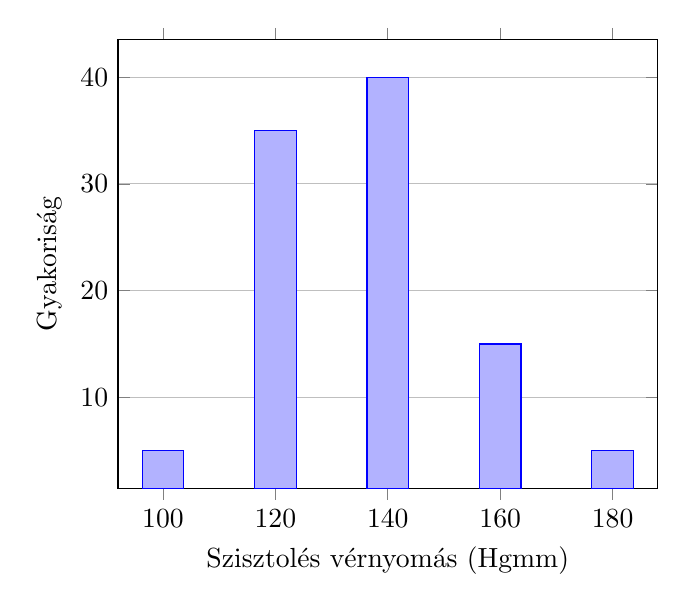
\begin{tikzpicture}
\begin{axis}[
    ybar,
    ylabel={Gyakoriság},
    xlabel={Szisztolés vérnyomás (Hgmm)},
    xtick={100,120,140,160,180},
    ytick={0,10,20,30,40},
    ymajorgrids=true,
    bar width=15pt,
]
\addplot coordinates {
    (100,5) (120,35) (140,40) (160,15) (180,5)
};
\end{axis}
\end{tikzpicture}
\end{center}

Ez a hisztogram mutatja, hogy a legtöbb érték 120-140 Hgmm között van, és az eloszlás közel szimmetrikus.
\end{description}

\subsubsection{Magfüggvényes sűrűségbecslés}

\begin{description}
\item[Példa:] Ugyanazon vérnyomásadatok magfüggvényes sűrűségbecslése:

\begin{center}
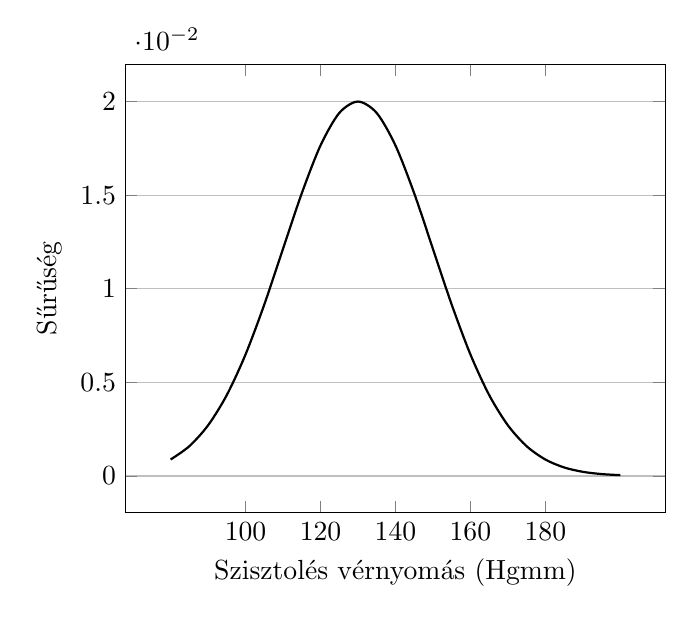
\begin{tikzpicture}
\begin{axis}[
    ylabel={Sűrűség},
    xlabel={Szisztolés vérnyomás (Hgmm)},
    xtick={100,120,140,160,180},
    ymajorgrids=true,
]
\addplot[smooth, thick, domain=80:200] {0.02*exp(-0.5*((x-130)/20)^2)};
\end{axis}
\end{tikzpicture}
\end{center}

Ez a becslés simább képet ad az eloszlásról, mint a hisztogram, és jól mutatja az eloszlás csúcsát 130 Hgmm körül.
\end{description}

\subsubsection{Tukey-féle boxplot}

A könyv a Low Infant Birth Weight (LOWBWT) adatbázis születési tömeg (bwt) változóját használja példaként a boxplot bemutatására.

\begin{description}
\item[Példa:] A LOWBWT adatbázis születési tömeg változójának boxplot ábrázolása:

\begin{center}
\begin{tikzpicture}
\begin{axis}[
    y=0.004cm,
    boxplot/draw direction=y,
    ylabel={Születési tömeg [g]},
    ytick={1000,2000,3000,4000,5000},
    height=8cm,
    width=6cm
]
\addplot+[
    boxplot prepared={
      lower whisker=709,
      lower quartile=2414,
      median=2977,
      upper quartile=3487,
      upper whisker=4990
    },
] coordinates {};
\end{axis}
\end{tikzpicture}
\end{center}

A boxplot értelmezése:
\begin{itemize}
    \item A doboz alja az első kvartilis (Q1 = 2414 g)
    \item A dobozban lévő vonal a medián (2977 g)
    \item A doboz teteje a harmadik kvartilis (Q3 = 3487 g)
    \item Az alsó "bajusz" vége a legkisebb nem kiugró érték (709 g)
    \item A felső "bajusz" vége a legnagyobb nem kiugró érték (4990 g)
\end{itemize}

Fontos megjegyzések:
\begin{itemize}
    \item Az interkvartilis terjedelem (IQR) = Q3 - Q1 = 3487 - 2414 = 1073 g
    \item A boxplot nem mutat kiugró értékeket ebben a példában
    \item Az eloszlás enyhén jobbra ferde, mivel a medián közelebb van Q1-hez, mint Q3-hoz
\end{itemize}
\end{description}

(Forrás: 32-33. oldal, 3.5. ábra)

\subsection{Két folytonos változó együttes vizsgálata}

Két folytonos változó kapcsolatának vizsgálatára több módszer is rendelkezésünkre áll. Ezek közül a legfontosabbak a kovariancia, a korreláció és a szóródási diagram.

\subsubsection{Kovariancia}

A kovariancia két változó együttes változékonyságát méri.

\begin{equation}
\text{cov}(x,y) = \frac{\sum_{i=1}^n (x_i - \bar{x})(y_i - \bar{y})}{n}
\end{equation}

\begin{description}
\item[Értelmezés:]
\begin{itemize}
    \item Pozitív kovariancia: a változók együtt mozognak
    \item Negatív kovariancia: a változók ellentétesen mozognak
    \item Nulla körüli kovariancia: nincs lineáris kapcsolat
\end{itemize}
\item[Hátrány:] Skálafüggő, nehezen összehasonlítható különböző változópárok között
\end{description}

(Forrás: 38-39. oldal)

\subsubsection{Korreláció}

A korreláció a kovariancia standardizált formája, amely -1 és +1 között mozog.

\begin{equation}
r = \frac{\text{cov}(x,y)}{s_x s_y}
\end{equation}

ahol $s_x$ és $s_y$ az $x$ és $y$ változók szórása.

\begin{description}
\item[Értelmezés:]
\begin{itemize}
    \item $r = 1$: tökéletes pozitív lineáris kapcsolat
    \item $r = -1$: tökéletes negatív lineáris kapcsolat
    \item $r = 0$: nincs lineáris kapcsolat
\end{itemize}
\item[Előnyök:]
\begin{itemize}
    \item Skálafüggetlen, összehasonlítható különböző változópárok között
    \item Könnyen értelmezhető
\end{itemize}
\item[Hátrányok:]
\begin{itemize}
    \item Csak lineáris kapcsolatot mér
    \item Érzékeny a kiugró értékekre
\end{itemize}
\end{description}

(Forrás: 39-40. oldal)

\subsubsection{Szóródási diagram}

A szóródási diagram két folytonos változó kapcsolatának grafikus ábrázolása.

\begin{description}
\item[Készítés:] Minden megfigyelési egységhez egy pontot rajzolunk egy derékszögű koordináta-rendszerben, ahol az x-koordináta az egyik, az y-koordináta a másik változó értéke.

\item[Példa:] Tekintsük az anyai testtömeg (lwt) és az újszülött születési tömege (bwt) közötti kapcsolatot a LOWBWT adatbázisban:

\begin{center}
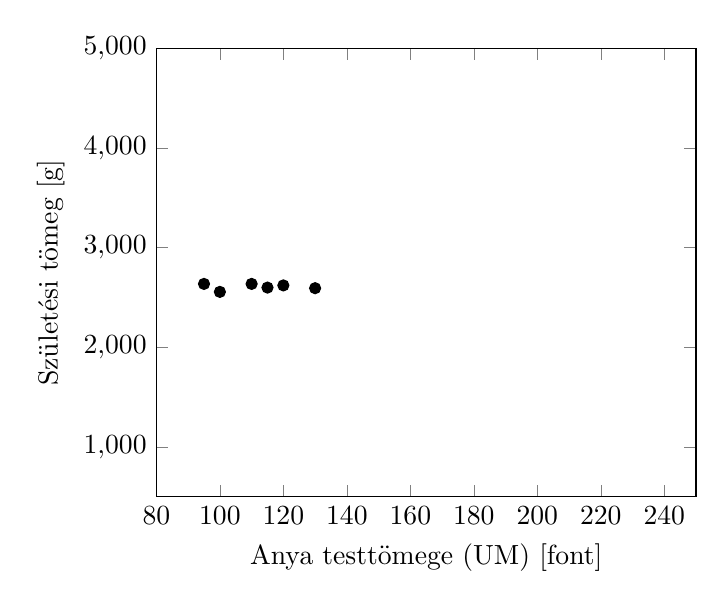
\begin{tikzpicture}
\begin{axis}[
    xlabel={Anya testtömege (UM) [font]},
    ylabel={Születési tömeg [g]},
    xmin=80, xmax=250,
    ymin=500, ymax=5000,
    scatter/use mapped color={draw=black, fill=black},
]
\addplot[only marks, scatter] table[x=lwt, y=bwt] {
lwt bwt
100 2557
130 2594
115 2600
120 2622
110 2637
95  2637
};
\end{axis}
\end{tikzpicture}
\end{center}

\item[Értelmezés:] 
\begin{itemize}
    \item A pontok elhelyezkedése mutatja a kapcsolat jellegét és erősségét
    \item Lineáris trend esetén a pontok egy egyenes mentén csoportosulnak
    \item A szórás mértéke az egyenes körül mutatja a kapcsolat erősségét
\end{itemize}

\item[Előnyök:]
\begin{itemize}
    \item Vizuálisan jól értelmezhető
    \item Nemlineáris kapcsolatokat is kimutat
    \item Kiugró értékek könnyen azonosíthatók
\end{itemize}
\end{description}

(Forrás: 40-41. oldal)

\end{document}





















